\begin{center}
    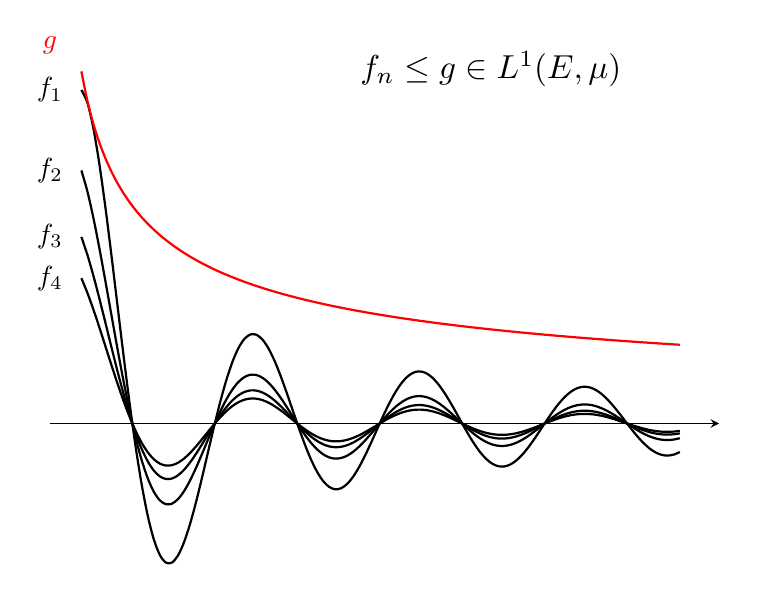
\begin{tikzpicture}
        \draw [-stealth] (0, 0) -- (8.5, 0) node[below] {};

        \foreach \n in {1, 2, 3, 4} {
                \draw[thick, domain=0.4:8, smooth, variable=\x, samples=100] plot ({\x}, {(10 * \n * sin(3 * \x r)) / (1 + \n^2 * 3 * \x)});
            }

        \foreach \n in {1, 2, 3, 4} {
                \node[scale=1] at (0, {(10 * \n * sin(3 * 0.4 r)) / (1 + \n^2 * 3 * 0.4)}) {\(f_{\n}\)};
            }

        \draw[thick, domain=0.4:8, smooth, variable=\x, samples=100, color=red] plot ({\x}, {(8 / \x)^(1/2)});
        \node[scale=1, color=red] at (0, 4.8) {\(g\)};

        \node[scale=1.2] at (5.6, 4.5) {\(\abs{f_n} \leq g \in \mc{L}^1(E, \mu)\)};
    \end{tikzpicture}
\end{center}

\section*{Almost Everywhere}

지난 글에서 measure가 0인 집합 위에서 적분하면 결과가 0이 됨을 확인했습니다. 적분 입장에서 보면 measure가 0인 곳에서의 적분은 의미가 없다고 생각할 수 있겠죠? 그러면 앞으로 그런걸 무시해도 된다고 하면 어떨까요?

\defn. \note{Almost Everywhere} \(P = P(x)\) 가 어떤 성질이라 하자.\footnote{예를 들어, `\(f(x)\)가 연속이다' 등.} 만약 measure가 0인 집합 \(N\)이 존재하여 성질 \(P\)가 모든 \(x \in E \bs N\) 에서 성립하면, \(P\)가 \(E\)의 \textbf{거의 모든 점에서} 성립한다고 한다.

\notation 위를 편의상 `\(P\) \(\mu\)-\ae (\textbf{almost everywhere}) on \(E\)'로 적겠습니다.

확률론과도 연관이 깊은 정리 하나를 소개하고 가겠습니다.

\thm. \note{Markov Inequality} \(u \in \mc{L}^{1}(E, \mu)\) 라 하자. 모든 \(c > 0\) 에 대하여
\[
    \mu\paren{\{\abs{u} \geq c\} \cap E} \leq \frac{1}{c} \int_E \abs{u} \d{\mu}
\]
이다.

\pf \(\ds \int_E \abs{u} \d{\mu} \geq \int_{E\cap \{\abs{u}\geq c\}} \abs{u} \d{\mu} \geq \int_{E\cap \{\abs{u}\geq c\}} c \d{\mu} = c \mu\paren{\{\abs{u} \geq c\} \cap E}\).

아래 정리는 measure가 0인 집합에서의 적분은 무시해도 됨을 알려줍니다. \(u(x) \neq 0\) 인 점들이 존재하더라도, 이 점들의 집합의 measure가 0이면 적분값에 영향을 줄 수 없습니다.

\thm. \(u\in \mc{L}^{1}(E, \mu)\) 일 때, 다음은 동치이다.
\begin{enumerate}
    \item \(\ds \int_E \abs{u} \d{\mu} = 0\).
    \item \(u = 0\) \(\mu\)-\ae on \(E\).
    \item \(\mu\paren{\{x \in E : u(x) \neq 0\}} = 0\).
\end{enumerate}

\pf \\
\note{2\(\iff\)3} \(E\cap\{u\neq 0\}\) 가 measurable이므로 정의에 의해 당연하다.

\note{2\mimp1} \(\ds \int_E \abs{u} \d{\mu} = \int_{E \cap \{\abs{u} > 0\}} \abs{u} \d{\mu} + \int_{E \cap \{\abs{u} = 0\}} \abs{u} \d{\mu} = 0 + 0 = 0\).

\note{1\mimp3} Markov inequality를 사용하면
\[
    \mu\paren{\left\{\abs{u} \geq \frac{1}{n}\right\} \cap E} \leq n\int_E \abs{u} \d{\mu} = 0
\]
이다. 이제 \(n\ra \infty\) 일 때 continuity of measure를 사용하면 \(\mu\paren{\{\abs{u} > 0\} \cap E} = 0\) 이다.

위 정리의 결과를 생각해 보면 다음이 성립함도 알 수 있습니다.

\rmk \(A, B\)가 measurable이라 하자. \(B \subset A\) 이고 \(\mu\paren{A \bs B} = 0\) 이면 모든 \(f \in \mc{L}^{1}(A, \mu)\) 에 대하여
\[
    \int_A f \d{\mu} = \int_B f \d{\mu}
\]
이다.

또한 적분값이 유한하다면, 거의 모든 점에서 함숫값이 유한해야 할 것입니다!

\thm. \(u \in \mc{L}^{1}(E, \mu)\) 이면 \(u(x) \in \R\) \(\mu\)-\ae on \(E\) 이다. 즉, \(u(x) = \infty\) 인 집합의 measure가 0이다.

\pf \(\mu\paren{\{\abs{u} \geq 1\}\cap E} \leq \ds \int_E \abs{u} \d{\mu} < \infty\).\footnote{Continuity of measure를 사용하기 위해서는 첫 번째 집합의 measure가 유한해야 한다.} 그러므로
\[
    \begin{aligned}
        \mu\paren{\{\abs{u} = \infty\} \cap E} & = \mu\paren{\bigcap_{n=1}^\infty \{x \in E : \abs{u(x)} \geq n\}}                                                           \\
                                               & = \lim_{n \ra \infty} \mu\paren{\{\abs{u} \geq n\} \cap E} \leq \limsup_{n\ra\infty} \frac{1}{n} \int_E \abs{u} \d{\mu} = 0
    \end{aligned}
\]
이다.

적분 가능하다면 어차피 함숫값이 무한한 영역은 적분값에 영향을 주지 않으므로, 함숫값이 유한한 곳에서만 적분해도 될 것입니다.

\cor \(u \in \mc{L}^{1}(E, \mu)\) 이면 \(\ds \int_E u \d{\mu} = \int_{E \cap \{\abs{u} < \infty\}} u \d{\mu}\) 이다.

드디어 일반적인 경우에서 적분의 선형성을 증명합니다!

\thm. \(f_1, f_2 \in \mc{L}^{1}(E, \mu)\) 이면 \(f_1 + f_2 \in \mc{L}^{1}(E, \mu)\) 이고
\[
    \int_E \paren{f_1 + f_2} \d{\mu} = \int_E f_1 \d{\mu} + \int_E f_2 \d{\mu}
\]
이다.

\pf \(\abs{f_1 + f_2} \leq \abs{f_1} + \abs{f_2}\) 임을 이용하면 \(f_1+f_2 \in \mc{L}^{1}(E, \mu)\) 인 것은 당연하다. 이제 \(f = f_1 + f_2\) 로 두고
\[
    N = \left\{x : \max\left\{f_1^+, f_1^-, f_2^+, f_2^-, f^+, f^-\right\} = \infty \right\}
\]
으로 정의하자. 함수들이 모두 적분 가능하므로 위 정리에 의해 \(\mu(N) = 0\) 이다. 그러므로 \(E \bs N\) 에서는 무한한 값이 없으므로 이항을 편하게 할 수 있다. 즉,
\[
    f^+ - f^- = f_1^+ - f_1^- + f_2^+ - f_2^- \implies f^+ + f_1^- + f_2^- = f^- + f_1^+ + f_2^+
\]
이다. 그러면
\[
    \int_{E\bs N} f^+ \d{\mu} + \int_{E\bs N} f_1^- \d{\mu} + \int_{E\bs N} f_2^- \d{\mu} = \int_{E\bs N} f^-\d{\mu} + \int_{E\bs N} f_1^+\d{\mu} + \int_{E\bs N} f_2^+ \d{\mu}
\]
이고, \(\mu(N) = 0\) 임을 이용하여 \(N\) 위에서의 적분값을 더해주면
\[
    \int_{E \bs N} f \d{\mu} = \int_{E \bs N} f_1 \d{\mu} + \int_{E \bs N} f_2 \d{\mu} \implies \int_{E} f \d{\mu} = \int_{E} f_1 \d{\mu} + \int_{E} f_2 \d{\mu}
\]
를 얻는다.

\dots

이제 이를 응용하여 수렴정리를 다시 적어보겠습니다. 지난 글에서는 모든 점에서 특정 성질이 성립할 것이 요구되었으나 이제는 거의 모든 점에서만 성립하면 됩니다. 증명은 해당 성질이 성립하지 않는 집합을 빼고 증명하면 됩니다.

\thm{11.28} \note{단조 수렴 정리} \(f_n\)이 measurable이고 \(0 \leq f_n(x) \leq f_{n+1}(x)\) \(\mu\)-\ae 라 하자.
\[
    \lim_{n\ra\infty} f_n(x) = f(x)
\]
로 두면,
\[
    \lim_{n \ra \infty} \int_E f_n \d{\mu} = \int_E f \d{\mu}.
\]
이다.

\thm{11.31} \note{Fatou} \(f_n\)이 measurable이고 \(f_n(x) \geq 0\) \(\mu\)-\ae 라 하자. 다음이 성립한다.
\[
    \int_E \liminf_{n\ra\infty} f_n \d{\mu} \leq \liminf_{n\ra\infty} \int_E f_n \d{\mu}.
\]

비슷한 느낌으로 다음과 같은 명제를 생각할 수도 있습니다.

\prop. \(E\) 위의 measurable function \(f, g\)에 대하여 \(\abs{f} \leq \abs{g}\) \(\mu\)-\ae on \(E\) 이면,
\[
    \int \abs{f} \d{\mu} \leq \int \abs{g} \d{\mu}
\]
이므로, \(g \in \mc{L}^{1}(E, \mu)\) 이면 \(f \in \mc{L}^{1}(E, \mu)\) 이다.

사실 \(\mu\)-\ae 를 정의한 이유가 또 있습니다. 이는 뒤에서 \(\mc{L}^p\) 공간을 공부하며 명확해질 것입니다. 두 함수 간의 거리를 정의한다면, 함수의 차를 적분한 값을 떠올릴 수 있을 것입니다. 그런데 거리 함수(metric) 정의상, 거리가 0이려면 거리를 잰 두 대상이 같아야 합니다! 그런데 르벡 적분의 경우 실제로 함수가 같지 않지만 거의 모든 점에서 함숫값이 일치하여 차의 적분값이 0이 되어버릴 수도 있습니다.

\defn. Measurable set \(E\)에 대하여, \(\mc{L}^{1}(E, \mu)\)의 함수에 대한 relation \(\sim\)을 다음과 같이 정의한다.
\begin{center}
    \(f \sim g \iff f = g\) \(\mu\)-\ae on \(E\).
\end{center}
그러면 \(\sim\)은 equivalence relation이고 다음과 같이 적을 수 있다.
\[
    [f] = \{g \in \mc{L}^{1}(E, \mu) : f \sim g\}.
\]

이처럼 equivalence relation을 정의하면 equivalence class의 대표에 대해서만 생각해도 충분합니다. 사실상 거의 모든 점에서 함숫값이 같다면 같은 함수로 보겠다는 뜻이 됩니다.

\section*{Dominated Convergence Theorem}

마지막 수렴정리를 소개하고 수렴정리와 관련된 내용을 마칩니다. 지배 수렴 정리(dominated convergence theorem, DCT)로 불립니다.

\thm{11.32} \note{지배 수렴 정리} Measurable set \(E\)와 measurable function \(f\)에 대하여, \(\{f_n\}\)이 measurable function의 함수열이라 하자. \(E\)의 거의 모든 점 위에서 극한 \(f(x) = \ds \lim_{n \ra \infty} f_n(x)\) 가 \(\overline{\R}\)에 존재하고 (점별 수렴)
\begin{center}
    \(\abs{f_n} \leq g \quad \mu\)-\ae on \(E\) (\(\forall n \geq 1\))
\end{center}
를 만족하는 \(g \in \mc{L}^{1}(E, \mu)\) 가 존재하면,
\[
    \lim_{n \ra \infty} \int_E \abs{f_n - f} \d{\mu} = 0
\]
이다.

\rmk
\begin{enumerate}
    \item \(f_n, f \in \mc{L}^{1}(E, \mu)\) 이다.
    \item 적분의 성질에 의해
          \[
              \abs{\int f_n \d{\mu} - \int f \d{\mu}} \leq \int \abs{f_n - f} \d{\mu}
          \]
          이므로 위 정리의 결론은 곧
          \[
              \lim_{n \ra \infty} \int f_n \d{\mu} = \int f \d{\mu}
          \]
          를 의미한다.
\end{enumerate}

\pf 다음과 같은 집합을 정의한다.
\[
    A = \left\{\ds x \in E : \lim_{n \ra \infty} f_n(x) \text{가 존재하고}, f_n(x), f(x), g(x) \in \R, \abs{f_n(x)} \leq g(x)\right\}.
\]
그러면 가정에 의해 \(\mu\paren{E\bs A} = 0\) 이다. 이제 \(x \in A\) 에 대해서만 생각해도 충분하다. 그러면
\[
    2g - \abs{f_n - f} \geq 2g - \bigl(\abs{f_n} + \abs{f} \bigr) \geq 0
\]
이다. \(\abs{f_n - f} \ra 0\), \(2g - \abs{f_n - f} \ra 2g\) 이므로, Fatou's lemma를 적용하면
\[
    \begin{aligned}
        2 \int_E g \d{\mu} = \int_A 2g \d{\mu} & = \int_A \liminf_{n \ra \infty} \big(2g - \abs{f_n - f}\big) \d{\mu}                               \\
                                               & \leq \liminf_{n \ra \infty} \paren{2 \int_A g \d{\mu} - \int_A \abs{f_n - f} \d{\mu}}              \\
                                               & = 2\int_A g \d{\mu} - \limsup_{n \ra \infty} \int_A \abs{f_n - f} \d{\mu} \leq 2 \int_A g \d{\mu}
    \end{aligned}
\]
이다. 따라서
\[
    2 \int_A g \d{\mu} - \limsup_{n \ra \infty} \int_A \abs{f_n - f} \d{\mu} = 2 \int_A g \d{\mu}
\]
이고, 가정에 의해 \(\ds 0 \leq \int_A g \d{\mu} < \infty\) 이므로 \(\ds \limsup_{n \ra \infty} \int_A \abs{f_n - f} \d{\mu} = 0\) 이다.

...

DCT를 사용하여 여러 흥미로운 결과를 얻을 수 있습니다. 다음 글에서는 DCT를 활용하여 리만 적분과 르벡 적분을 비교하도록 하겠습니다.
